\FloatBarrier

\subsection{Standard Optical Technologies}

This section describes several optical technologies, such as for instance laser and signal
detection systems, required for the realisation
of any interferometric gravitational wave detector.  In the following we refer to
these techniques as 'standard optical technologies' because when building ET
we will be able to rely on ample experience in these technologies collected 
from commissioning and operating the first and second generation of gravitational wave
detectors. 

In section~\ref{sec:injection} we describe the ET injection system consisting 
of the pre-stabilised lasers and the input mode cleaners. The readout of the 
gravitational wave signal and the design options for output mode cleaners are 
discussed in section~\ref{sec:detection}. Section~\ref{sec:control} gives an 
general overview on how to control the main optical components of ET for 
their longitudinal and angular degrees of freedom. Finally section~\ref{sec:tcs}
describes strategies to mitigate the effects of thermal lensing by means of 
thermal compensation. 


\FloatBarrier
\subsubsection{Injection system}\label{sec:injection}
%\emph{Author(s): P. Wessels, E. Genin and S. Hild \\}

\etbox{h}{hbox:IO_requirements}{Laser beams required at the input of the main interferometers}
{\begin{table}[H]
\centering
\color{\contentcolor}
\begin{tabular}{c|c|c}
\hline
\hline
 & ET-HF &ET-LF\\
\hline
Wavelength &1064\,nm  & 1550\,nm\\
Beam shape & Laguerre Gauss 3,3   & TEM$_{00}$  \\
Optical power in front of  PRM & 500\,W& 3\,W\\
\hline
\hline
\end{tabular}
\end{table}
}

\FloatBarrier
\paragraph{Pre-stabilized laser}

At the development time of second generation GWDs, Neodymium doped Yttrium Aluminium garnet (Nd:YAG) was the best choice as the gain material for 100~W class lasers. However, in the last years, particularly thin disc lasers based on Ytterbium doped crystals have been undergoing a rapid development. The pure power scaling of these systems into the multi-kW range was mainly driven either by material processing or defense applications \cite{Deile2009,Kalisky2010}, which do neither require single-frequency nor fundamental mode output. Nevertheless, good progress has also been achieved in the power scaling of high beam quality laser systems. In particular, near fundamental mode operation with more than 200~W of output power and up to 98~W of single-frequency output power has been demonstrated \cite{Giesen2007}. Further possible advantages are that the 940~nm pump diodes used for e.g.\ Yb:YAG have potentially longer lifetimes than their 808~nm Nd:YAG counterparts and that the lower quantum defect of Yb:YAG causes less thermal effects. However, Yb:YAG is a quasi-3-level system and thus its main disadvantage is that it is more sensitive to increased temperatures within the gain medium.

In order to produce lasers with power levels of several 100~W and to amplify these systems into the kW region, different design concepts are proposed. The main concerns are the thermal management in the gain material and to reduce beam aberrations. In particular, Nd:YAG suffers from a significantly higher quantum defect compared to Yb:YAG making the thermal management even more important. One way to reduce the thermal effects is to use a zig-zag beam path to average over the thermal gradient in the laser crystal. Edge-pumped slab geometries can be combined with conduction-cooling techniques, which avoid vibrations introduced by cooling fluids in conventional layouts. However, one of the main challenges in using slabs is to avoid parasitic oscillations within the high gain regions.

Problems caused by depolarisation and by defocusing can be addressed in different ways. In principle, an efficient birefringence compensation can be implemented~\cite{Lue1996}. However, better than compensating effects is to reduce these. For this, there are in principle two different options. Firstly, \citet{Koechner1971} and \citet{Soms1980} have shown that the amount of depolarisation depends on the Nd:YAG crystal orientation. Therefore, crystal orientations other than the standard [111]-cut could be an option to reduce the depolarisation intrinsically. \citet{Shoji2002} suggested the use of [110]-cut crystals in combination with small beam size in the high pumping regime to reduce depolarisation. In recent experiments~\cite{Puncken2010}, the [100]-, [110]- and [111]-crystal orientations were compared in a single pass configuration in the pump power regime relevant for 2nd generation GWD. Although these results are very promising in terms of intrinsic reduction of depolarisation effects, they also show that the non-symmetrical shape of the thermal lens in unconventionally cut crystals might limit the achievable beam quality in laser oscillators.

The second option is to reduce the thermal gradients which cause these stress-induced birefringence effects. As shown in the work by \citet{Wilhelm2009,Wilhelm2010}, the maximum peak temperature of an end-pumped laser rod or slab can be reduced by the use of laser rods composed of several segments with different doping concentrations. 
The quantum defect and therefore the overall heat load in a Nd:YAG laser media can be reduced by more than 30\% by changing the pump wavelength from 807~nm to 885~nm (see e.g.~\cite{Lavi2000,Frede2006}).
Core doped rods can be used (see e.g.~\cite{Kracht2006}) to achieve an easier and more stable fundamental mode operation.
In these rods only the inner core is doped and the outer core is used as a waveguide for the pump light comparable to a double clad fibre as described by \citet{Bedoe1993}. This concept is similar to mode selective pumping as the gain is only present in the doped inner core of the rod. However, it has the advantage that no high brightness pump source is required.

Optical fibre amplifiers have a large potential to offer single-frequency output at higher efficiencies and lower cost than solid-state amplifiers at similar power levels (see for example the overview paper by~\citet{Limpert2007}). Until several years ago, diode-pumped fibre amplifiers were limited to power levels of several Watts. This was both due to the unavailability of high brightness pump diodes as well as due to nonlinear effects in the fibre such as stimulated Raman scattering and stimulated Brillouin scattering (SBS).
The invention of large mode-area (LMA) fibres and of photonic crystal fibres (PCF) has enabled output powers of single-mode fibre lasers to exceed 1~kW while retaining excellent efficiencies (see for example~\citet{Jeong2004}). The large effective core diameter of these fibres decreases the average intensity of the light at the laser wavelength in the fibre and thereby increases the threshold of nonlinear processes. The large inner cladding of the double-clad LMA fibres allows high power multi-mode pumps to be coupled into the fibre. Despite the large diameter of the active core, a clean single-mode output can be obtained by suppressing the higher order transverse modes by bending losses. A typical PCF geometry and a representative beam profile of such a fibre is shown in Fig.~\ref{fig:pcf_geometry}. The limiting factor for \emph{narrow-linewidth} high-power fibre lasers for the use in GWDs is the onset of SBS.

\begin{figure*}[h]
\begin{center}
  \begin{tabular}[c]{c}
    \includegraphics[width=0.4\textwidth]{./Sec_Optics/sem_picture_pcf}
  \end{tabular}
  \hspace*{1cm}
  \begin{tabular}[c]{c}
    \includegraphics[width=0.25\textwidth]{./Sec_Optics/beamprofile_pcf}
  \end{tabular}
  \caption{Typical geometry of a large-core photonic crystal fibre (left) and typical beam profile (right).}
  \label{fig:pcf_geometry}
\end{center}
\end{figure*}

A state-of-the art single-frequency fibre amplifier system with 150~W of output power with a good output beam profile (92\% in TEM$_{00}$) is described in~\cite{Hildebrandt2006}. With this system an optical-to-optical efficiency of 78\% with respect to incident pump power was achieved with a good polarisation ratio of about 100/1. Recently, the output power of single-frequency, PCF-based, Ytterbium-doped fibre amplifiers has been scaled to more than 400~W of output power \cite{Robin2010}.

A different approach to realize LMA fibres with excellent output beam quality and simultaneously larger mode areas are multifilament-core (MFC) fibres with core regions consisting of many small doped filaments.  In contrast to conventional multi-core design, the multifilament core fibres aim for strong coupling between smaller filaments resulting in the propagation of only one supermode by adequately choosing the diameter and spacing of the filaments. In the last years, MFC fibres with active and also with passive filaments were demonstrated, which enabled transversely single-mode output with a nearly Gaussian-shaped intensity mode profile~\cite{Canat2008,Vogel2009}. The main advantage of this new fibre type is the low effective core numerical aperture which can be achieved without the need for flattening the refractive index profile as it is crucial for PCFs. This is of particular importance for large index core materials like Erbium-Ytterbium codoped fibres for which this design approach allows for a precise reduction and control of the effective core index. Important properties of the MFC fibres, e.g.\ the low bending losses, can be explained using an equivalent step index based on the theory of the fundamental space filling mode~\cite{Canat2010}. Recently, it has been demonstrated that a TEM$_{00}$ mode content of more than 95\% can be achieved with such an actively doped fibre~\cite{Kuhn2010}. In Fig.~\ref{fig:mfc_mode}, both the calculated as well as the measured mode profile of an Erbium-Ytterbium codoped MFC fibre with 37 filaments is shown.

\begin{figure*}[h]
\begin{center}
  \begin{tabular}[c]{c}
    \includegraphics[width=0.45\textwidth]{./Sec_Optics/mfc_mode_calc.png}
  \end{tabular}
  \hspace*{1cm}
  \begin{tabular}[c]{c}
    \includegraphics[width=0.25\textwidth]{./Sec_Optics/mfc_mode}
  \end{tabular}
  \caption{Calculated mode profile for an Er-Yb multifilament-core fibre with 37 filaments (left) and measured mode profile (right) with a fundamental Gaussian mode content of more than 95\%.}
  \label{fig:mfc_mode}
\end{center}
\end{figure*}

Novel ideas to increase the SBS threshold are under investigation. A promising concept is to shift the Brillouin frequency along the fibre to lower the effective Brillouin gain for each frequency component. This could be achieved by temperature or strain gradients, or by varying doping concentrations along the fibre.
Furthermore, fibres with specially designed transverse refractive index profiles are being developed to minimize the overlap of the optical and the acoustical fibre modes, also resulting in an effective reduction of the Brillouin gain.

Besides the power scaling aspect, the reliability and noise performance of high power fibre lasers need to be further analyzed and possibly improved to meet the requirements of third generation gravitational wave detectors. Especially thermal effects and contamination at the air-glass interface have to be considered. The main problem is the large light intensity at these interfaces which could be reduced by use of an undoped beam expansion section at the fibre ends or by all-fibre solutions for the pump-light coupling. One big advantage of fibre lasers is that they are compact and simple compared to the complex solid-state laser systems. Furthermore, modern splice techniques allow to produce monolithic all-fibre systems including the master oscillator, the high power stage and possibly even a mode-cleaning fibre, if required.

Erbium-doped fibre lasers emit around 1.56~$\mu$m where the absorption in silicon is small compared to the silica substrates currently used at 1~$\mu$m wavelength. For an efficient design with low nonlinear effects in single frequency operation, the Erbium-doped fibre should have high pump absorption and should be as short as possible. Unfortunately, the pump absorption cross sections of Erbium are about a factor of 10 lower than those of Ytterbium. In addition, quenching effects also limit the sensible doping concentrations to about a factor of 10 below that of Ytterbium. These combined factors result in about two orders of magnitude lower pump absorption of Erbium doped fibres, if similar fibre geometries as used with Ytterbium doped fibres are assumed. In order to avoid excessive fibre lengths, which is necessary to circumvent the onset of SBS, either the signal-core to pump-core ratio has to be adapted or the amplifier even has to be pumped into the single-mode signal core. For these reasons, pump sources with very high brightness or even single-mode beam quality are needed. This becomes even more obvious if the typically achieved optical-to-optical efficiencies of about 25\%--30\% (50\% for 1480~nm pumping) are compared with the typical value of ${}>70\%$ for Ytterbium. Recently, a single-mode output power of 81~W at 1480~nm was demonstrated with a Raman fibre laser~\cite{Nicholson2010} which can be used as a pump source for single-mode Er based systems. However, commercially available single-mode Raman fibre laser modules are currently limited to an output power of 10--20~W.

In order to overcome these limitations, Yb codoping of Er-doped fibres and pumping at 980 nm can be used. This allows high pump absorption but also implicates a second gain band at the Yb wavelength around 1~$\mu$m. This second gain bands limits the achievable output power due to the onset of massive amplified spontaneous emission (ASE) which finally leads to pulsing instabilities of the amplifier system. The highest single-frequency output power of 151~W achieved with this concept was accompanied by more than 70~W of ASE at 1~$\mu$m~\cite{Jeong2005}. Nevertheless, in recent experiments a new scheme was demonstrated by which the 1~$\mu$m oscillation in an Er-Yb codoped fibre amplifier could be effectively suppressed~\cite{Kuhn2009}.

Concerning the direct generation or the amplification of spatial beam profiles other than the fundamental (fibre) mode, only very limited experimental results have been published. A good overview is given in the review article by~\citet{Ramachandran2008}. For the generation of specific higher order modes, the laser light is first coupled into the fundamental LP$_{01}$ mode of a single-mode fibre. Then, an in-fibre long-period Bragg grating converts the LP$_{01}$ into the desired LP$_{0m}$ mode. This process can be very efficient with peak efficiencies of more then 99\%. The usage of higher order modes in the optical fibres has several advantages compared to the fundamental mode. Firstly, the effective mode area is significantly enlarged and hence the threshold for SBS is increased. Furthermore, the higher order modes are less sensitive to mode distortions due to fibre bending or refractive index profile imperfections due to the fibre fabrication process. Recently, fibre amplifiers have been demonstrated employing this technique for the first time in an active fibre with several Watts of output power~\cite{Nicholson2010a,Nicholson2010b}. However, all higher order LP$_{0m}$ modes used have a central high intensity peak in common which is undesirable for the use in GWD~\cite{Vinet2009}. Thus, some research on the generation of axisymmetric fibre modes with an intensity minimum in the centre as well as on the amplification of these modes will have to be carried out. Most probably, this will also involve some special design of active fibres in which the active dopant distribution favors the amplification of the mode of interest.

\etbox{r}{rbox:lasers}{Lasers for ET}
{
While the step from first to second generation gravitational wave detectors required
to scale the laser systems up by about a factor of 20, the step from second generation
to ET will only require a much smaller scaling factor of about 4 for ET-HF.
Research programs on ET lasers are already under way and no fundamental limits are known
which are expected to prevent the realisation of the high power laser for ET-HF.
The laser power
required for ET-LF is with only about 5\,W very small and currently already available.
}

\FloatBarrier
\paragraph{Injection optics}


%\textbf{Overview and General requirements}

The Input Optics system (IO) of ET takes care of the optics downstream of the lasers. The whole system must deliver a beam with the required power, geometrical shape, frequency and angular stability at the Interferometer input.




%
%%\bigskip
%\begin{table}[h]
%\centering
%%\begin{center}
%\begin{tabular}{l l l}
%\hline \hline
%{\bf Requirement} & {\bf Value at 1064 nm} & {\bf Value at 1550 nm}\\
%\hline
%Laser power available at the interferometer input & 500\,W   & 3\,W\\
%\hline
%Intensity noise & TBD & TBD\\
%\hline
%Beam jitter noise (misalignment mode amplitude) & TBD & TBD\\
%\hline
%IMC cavities throughput & $>80\%$ on LG$_{33}$ & $>80\%$ on TEM$_{00}$\\
%\hline
%IO overall throughput & $>50\%$ on LG$_{33}$ & $>50\%$ on TEM$_{00}$\\
%\hline \hline
%\end{tabular}
%%\end{center}
%\caption{Requirements for the ET Input Optics (IO) system \label{table:ET-IO}}
%\end{table}
%%\bigskip

Electro-Optic Modulators (EOM) should provide the needed RF phase or amplitude modulations
(to sense longitudinal and angular degrees of freedom; see section \ref{sec:control}). Two in-vacuum suspended input mode cleaners (IMC)
in series will be used to geometrically clean the beam and reduce its amplitude fluctuations as well as geometrical fluctuations. The
resonant IMC could also serve in the loop of laser frequency stabilization. After the IMC an intensity stabilization
section will provide the signal for stabilizing the laser's relative intensity noise (RIN)
and reach the requirements. An in-vacuum Faraday
isolator (FI) will prevent interaction of the interferometer reflected light with the IMC and laser system. Finally, a mode matching telescope will be used to
provide a beam with the correct size and wave front curvature  for matching it into the interferometer.
It is planned to use super-polished optics for ET-HF and ET-LF in order to lower as much as possible potential diffused
light noise.
Moreover the beam pointing noise created in components in free-space propagation (mirrors, lenses, EOM, FI,
etc.) can be dominated by acoustic, seismic and thermal noise. Particular effort will be given to isolate
the optics from seismic noise. Furthermore, several sensors used in the control loops will be placed on
suspended benches inside the vacuum vessel of ET.

\paragraph{Input Mode Cleaner}

The laser light must be frequency- and spatially stabilized before it can be used in the interferometer.
 The input mode cleaner  provides active frequency stabilization through feedback to the laser and passive
frequency noise suppression above its cavity pole frequency. %, and passive spatial stabilization at all frequencies.
The input mode cleaner also reduces higher order modal content of the laser light, suppressing beam jitter by a
factor depending of the cavity finesse.

%\subsection{IMC for ET-HF}

The baseline configuration of the IMC for ET-HF is to use two 20-meter
long IMC cavities placed in series (as done in GEO interferometer).
Due to the high laser power that will be stored in the IMC cavity,
radiation pressure effects and absorption in the  IMC cavity
input and output mirrors will be the main limiting effects. The radiation pressure effects
 will depend on the cavity
finesse chosen. In Advanced Virgo, with about 60\,kW power stored in this
cavity it has been shown that the radiation pressure effect on the angular
degrees of freedom is manageable by using mirrors of at least 3\,kg weight~\cite{RPnote}.
This means that this effect could be overcome by increasing the IMC
mirror weight or reducing the finesse if possible. For
the lock acquisition of the cavity it is likely that we need to lock the
cavity at a lower power and go to full power once the
cavity is locked~\cite{RPnote}. Radiation pressure noise (linked to
power fluctuation in the cavity) could also be responsible
for frequency noise since it can affect the length of the IMC cavity
and the angular control of the IMC end mirror if the beam
 is not well centered on this mirror. In the linear regime, it has been
 shown that radiation pressure noise was not an issue for
initial Virgo sensitivity~\cite{RPnoise} and Advanced Virgo~\cite{INJPDS}.
%Specifications on this noise will have to be given for ET.
Concerning input and output mirrors absorption, in order to
avoid beam distortion induced by photothermal effects, a low-absorption
fused silica grade with good homogeneity should be
chosen as mirror substrate and coating absorption lower than 1
ppm is mandatory~\cite{IMCcharac}.
In order to cope with higher order Laguerre-Gauss modes,
the resonant mode cleaner should be made with an even number
of mirrors as explained in~\cite{barsu,chelkow}.
Cavity parameters (finesse, round-trip losses and cavity pole)
will have to be defined according to the beam jitter, amplitude
and frequency noise requirements at the interferometer input.

%\subsection{IMC for ET-LF}

There are two main differences between the input mode cleaners for ET-HF and ET-LF:
First of all the optical power in the ET-LF IMC will be orders of magnitude
lower than in the ET-HF IMC and therefore we expect to encounter fewer potential issues
related to radiation pressure and thermal effects in the ET-LF IMC.
 Secondly the laser wavelength of the ET-LF IMC will
be 1550\,nm, which will allow us to strongly profit from
synergies with the telecommunication sector. Therefore, we believe the realisation
of the ET-LF IMC to be less challenging than the IMC for the ET high frequency interferometers.

%Due to the fact that a number of things have been developed in the 1550\,nm
%wavelength range for telecommunications, we will
%try to use as much as possible of the already existing components for the
%IMC of the ET-LF interferometers.
%For ET-LF, we have 2 possibilities to make a spatial filtering of the laser beam:
%\begin{itemize}
%\item use a resonant mode-cleaner as done in ET-HF
%\item use an optical fibre.
%\end{itemize}
%Some R\&D activity is needed on this subject to see if the optical fibre
%is able to fulfill ET requirements. In any case, a resonant cavity will
%probably be needed at least to stabilize the laser frequency.
%The baseline solution remains to use two 20-meter long triangular cavities
%in series where we have more experience and know that this kind of
%suspended cavity will fulfill our requirements.
%As for ET-HF, IMC parameters should be defined according to beam
%stability, laser frequency and amplitude stability required at the interferometer input port.

\paragraph{Faraday isolator}

In order to avoid unwanted cross-coupling, light back-reflected by the interferometer should
be picked up before being coupled back in the IMC cavities. The solution adopted in first
and second generations of gravitational wave detectors is to install a Faraday isolator in
vacuum on the beam path between the interferometer and the input mode cleaner cavity.

\emph{Faraday isolator for ET-HF:}
Faraday isolator designs have evolved to cope with the increase of power between first
and second generation detectors. A R\&D program put in place at the European Gravitational
Observatory in collaboration with the Institute of Applied Physics (Nyzhni Novgorod Russia) has
developed a Faraday isolator with reinforced magnetic field and using a thermal depolarization
 compensation technique~\cite{Khazanov_compensation}. This isolator uses Terbium Gallium
 Garnett (TGG) as magneto-optic material and the design has been optimized for thermal
 depolarization, thermal lensing and Verdet constant change compensation~\cite{HPIOfinal}.
 This device is able to achieve very good isolation performances (${}>38$\,dB) in vacuum from
 low power up to 250\,W laser power~\cite{genin}.
We could use this experience and the same kind of design and scale it up to get the expected
performances of the Faraday isolator in the 1\,kW power range.
For ET-HF we could expect that the in-vacuum Faraday isolator should have the following characteristics:
\begin{itemize}
\item withstand high average power (1\,kW) on long periods;
\item an optical isolation higher than 30\,dB at full power;
\item residual thermal lensing resulting in a focal length higher than 100\,m;
\item provide good transmission (at least 95\%)
\end{itemize}

\emph{Faraday isolator for ET-LF:}
In the telecom wavelength range, TGG cannot be used due to its higher absorption at 1550\,nm. Fortunately,
in the field of telecommunications a lot of possible materials are available that can
 be used for Faraday isolators~\cite{mavalvala}. The main aspect that needs to be checked
 for ET-LF is ultra-high vacuum compatibility of a 1550\,nm Faraday isolator.


 % In any case, as for the high power Faraday isolator needed for ET-HF, the development of vacuum compatible Faraday isolator for 1550\,nm wavelength requires to build up a test facility and collaborative work with laboratories or companies having experience with free space Faraday isolator adapted to telecom wavelength. The relatively low power used in the configuration will probably simplify the design of such an isolator with respect to the ET-HF high power Faraday isolator.

\paragraph{RF-Electro optical modulation system}
\nopagebreak

In ET radio-frequency (RF) modulation of the laser beam will be used in the control of the interferometer, both for longitudinal and angular controls.

\emph{RF modulation system for ET-HF:}
The main difference between the Electro Optical Modulation (EOM) system to be used in ET-HF respect to first and
second generation detectors is the laser power that the EOM system will have to withstand (up to 1\,kW for ET-HF).
Thermal effects become more significant~\cite{Mansell} and the choice of an appropriate material (electro-optic  crystal)
 becomes crucial to limit the consequences of these thermal effects on the EOM performance. Indeed, it is
 important to select the right material not only to limit wavefront aberrations but also to reduce local temperature fluctuations
 of the material. This heating can induce slow variations of the modulation index and therefore disturb the interferometer control.
The ET requirements  for the electro optical modulation system (oscillator phase noise, modulation index and modulation
index noise) will have to be defined in the technical design, as many of these parameters will affect the driving electronics and signal generator choice.

\emph{RF modulation system for ET-LF:}
The experience of telecommunication field will be used extensively in the RF-modulation system of ET-LF. It is likely that integrated fibered optical components will be used to modulate the laser light.

\paragraph{Other high power compatible components}
\nopagebreak

The selection and development of high power compatible components suitable for ET-HF is essential. Experience acquired during the Advance Virgo highpower input optics R\&D program should be a good starting point in the selection of waveplates, polarizers and for the design of high power low diffusing beam dumps~\cite{HPIOfinal,genin}.

%\paragraph{R\&D work needed for ET}
%\nopagebreak
%
%Laser and injection optics of ET can benefit of the many years of R\&D already performed within the  Advanced LIGO, Advanced Virgo and GEO-HF
% projects in investigating high power compliant components such as electro-optical modulators and Faraday isolators.
%
%For ET it is necessary to carry out the following two R\&D programs: the first one will be focussed on ET-HF components
%that have to be compliant with high power laser and the LG$_{33}$ mode. The second one should concern ET-LF and the
%development and selection of IO components (Faraday isolator, EOM, mirrors, waveplates and polarizers). Laser beam
% cleaning through a fiber has also to be studied for this configuration.
% %Collaboration with experienced people (laboratories
% %or companies) is essential in the success of these two R\&D programs.



\FloatBarrier
\subsubsection{Detection system}\label{sec:detection}
%\emph{Author(s): S.\ Hild and R. Goauty \\}
Traditionally detection system of first and second generation gravitational wave detector includes all
optical elements downstream the main interferometer (i.e. behind the signal
recycling mirror), such as for instance the readout photodiodes and the output mode
cleaner (OMC). In contrast,  as described already described in section~\ref{subsec:QNRsqz}
ET will feature the injection of frequency dependent squeezed light from the back of the interferometer
and there are lots of hardware components required for this purpose, such as for instance the squeezed light sources
as well as the filter cavities. In this section we will focus on the traditional components of a the detection
subsystem, i.e. the readout of the main gravitational wave signal and the output mode cleaner. 

\FloatBarrier
\paragraph{Readout options for the gravitational wave signal}

\begin{figure}[th]
\centering
\includegraphics[width=1\textwidth]{Sec_Optics/homo_hetero_schematic.pdf}
\caption[Different readout methods of a Michelson interferometer]{Illustration of three different 
readout methods of a Michelson interferometer:
heterodyne, homodyne and DC-readout. A detailed explanation is given in the text.}
\label{fig:principle}
\end{figure}


Figure~\ref{fig:principle} shows simplified schematics of three different readout
methods applied to a basic Michelson interferometer. Usually Michelson
interferometers used for gravitational wave detection are operated at the dark
 fringe, which  has the advantage
 of providing good suppression of common mode noise and allows to 
make use of power recycling.
The differential arm-length is controlled
to give destructive interference at the output port: ideally
 no carrier light ($f_{\rm c}$, red solid line) reaches the photo detector.
 A change of the differential arm length causes phase modulation
sidebands, i.e. gravitational
wave signal sidebands (blue dashed line). In contrast to the carrier light the gravitational
wave signal sidebands
 interfere constructively at the beam splitter, exit the interferometer towards its output port
and finally reach the photo detector.
The absolute frequency of the gravitational signal sidebands is given
 by $f_{\rm sig} =  f_{\rm c} \pm f_{\rm gw}$, where $f_{\rm gw}$ is the
 frequency of the gravitational wave (usually in the audio-band) and $f_{\rm c}$ 
the frequency of the main laser light (carrier).
Since $f_{\rm sig}$ is
a few hundred terahertz, the photodiode cannot directly detect
the gravitational wave signal, unless the presence of an optical local oscillator
is ensured. Heterodyne, homodyne and DC-readout are three different concepts to
ensure the presence of a low-noise optical local oscillator at the output port photodiode.


In the heterodyne scheme, commonly used by the first generation
gravitational wave detectors,
 radio frequency  sidebands ($f_{\rm het}$, green dotted lines)
are modulated onto the light at the input of
the Michelson interferometer (Schnupp modulation \cite{Schnupp1988}).
Introducing a macroscopic arm length difference of several centimeter
 (so-called Schnupp asymmetry) allows the modulation
sidebands to be transferred through the interferometer to the output port,
where they serve as optical local oscillator for the differential arm length  signal.
The photo-current produced by the beat between the different optical
field components (optical demodulation) contains
a radio frequency component at $f_{\rm het} \pm f_{\rm gw}$. In a second demodulation
process the photo-current is then electronically demodulated at $f_{\rm het}$ 
 in order to finally derive a signal stream at $f_{\rm gw}$.


In the homodyne readout scheme (center plot of Figure~\ref{fig:principle}) a  small
fraction of the carrier light is split off in front of the interferometer and guided directly
to the output photo detector without passing through the interferometer.
The big
advantage of this form of homodyne readout is that a phase shifter,
 placed in the local oscillator path, allows an easy
change of the optical demodulation phase, i.e.\ the readout quadrature,
without any hardware changes. On the other hand homodyne
readout has the disadvantage that the length and the alignment of the local-oscillator path needs to be highly stable.
In practice this usually implies that the local-oscillator path length as well as its alignment need to be actively
stabilized by a low-noise control system, and all components of the local-oscillator path must be
 seismically isolated inside a vacuum system.
Due to these demanding noise and hardware requirements, so far there have
been no serious plans to change
the readout scheme of the currently operating gravitational wave detectors
from heterodyne to homodyne readout.


DC-readout is a special case of homodyne readout which
is much easier to combine with the existing elements of  currently used
gravitational wave detectors.
In a DC-readout  scheme the operating point of the Michelson interferometer is slightly
shifted off the dark fringe, by introducing a so-called \emph{dark-fringe offset},
thus a certain amount of carrier light leaves the interferometer at the output port
 and can serve as local oscillator. Compared with the previously described homodyne readout,
DC-readout has the advantage that no additional local oscillator path outside the main interferometer
is required. On the other hand, DC-readout offers no easy way to vary the phase of the
optical demodulation.

DC-readout was already used in the first `Michelson' interferometer ever by Michelson and Morley
in 1887~\cite{michelson1887}. It is probably the simplest way to read out a Michelson
interferometer, but was considered to be unsuitable for the first generation of gravitational
wave detectors due to the strong coupling of laser power noise. However, increased
stability of the laser power inside future instruments gives hope for a renaissance
of DC-readout for gravitational wave detectors, which was first proposed
by Fritschel~\cite{Fritschel2}. 

The next section briefly summarises the general advantages and disadvantages of
DC-readout compared with heterodyne readout, especially taking into account the implications
for an interferometer with tuned or detuned signal recycling \cite{Hildtuned_detuned2007}.

\FloatBarrier

\etbox{i}{ibox:DC-readout}{Motivation for using DC-readout in ET}
{
DC-readout has several advantages over heterodyne
readout:
\begin{enumerate}
\item
DC-readout provides an increased 
signal to shot noise ratio compared to heterodyne readout \cite{Buonanno2003}. This is 
due to the fact that in the homodyne detection the shot noise contribution from frequencies 
twice the heterodyne frequency 
does not exist. 
\item
In DC-readout a reduced number of beating light fields at the detection port potentially reduces and 
simplifies the cross-couplings of technical noise \cite{Hildtuned_detuned2007}. Especially 
the coupling of amplitude and phase noise of the heterodyne modulation is 
strongly reduced in a DC-readout scheme. 
%\item
\item
A simpler calibration procedure can be applied for DC-readout, because the GW-signal is present in a single
data-stream even for
detuned signal-recycling (and not spread over the two heterodyne quadratures as
described in~\cite{Hewitson05}).
\item
As with DC-readout the main photodiode(s) and electronics for the detection do not need to be capable of
handling RF signals, they can be simplified.
\item
Large-area photodiodes may be used in DC-readout. These should offer reduced coupling of beam-pointing 
noise, due to decreased beam clipping and decreased influence of 
photo diode inhomogeneity (by averaging over a larger area). 
\item
As in the DC-readout configuration the local oscillator and the GW-signal pass the same optical system an 
optimal spatial overlap is guaranteed. (Due to thermal distortion current GW detectors 
employing arm cavities encountered the problem of imperfect spatial overlap of the carrier light 
(GW signal) and the heterodyne sidebands (local oscillator) \cite{Lawrence03})
\item Finally, the realization of a squeezed light enhanced
interferometer is simpler using DC-readout rather than heterodyne
readout. DC-readout requires squeezed light to be present only at
frequencies in the GW signal bandwidth compared to heterodyne
readout which requires squeezed light around twice the heterodyne
frequency as well~\cite{CDRGBM98}.
%\footnote{A squeezed light
%source working only in the GW signal bandwidth would result in the
%DC-readout case in a sensitivity enhancement limited by the squeezing
%strength generated, whereas the same source would act in a
%heterodyne-readout based interferometer as if 50\% of the squeezing
%was reduced due to losses. Hence, a sensitivity improvement by a
%factor of 6\,dB in the DC-readout case would result in the heterodyne
%case in an improvement factor of only 2\,dB.}
\end{enumerate}
}
%
This long list of advantages has to be compared with the drawbacks of DC-readout.
Even though power fluctuations of the carrier light (i.e. the local oscillator) 
are strongly filtered by the cavity poles of the power recycling cavity and the 
high-finesse arm cavities, the major disadvantage of DC-readout is  an
increased coupling of laser power noise. For the Einstein Telescope the advantages
of DC-readout clearly way out the disadvantages and therefore DC-readout was chosen as 
baseline configuration for the gravitational wave readout.


Recently enhanced LIGO and GEO-HF have successfully demonstrated the application
of DC-readout in long-baseline gravitational wave detectors. Furthermore, all advanced 
gravitational wave detectors plan to use DC-readout for the gravitational wave 
signal. Therefore, the commissioning of Advanced LIGO and Advanced Virgo is expected to greatly inform 
the technical design of the ET readout system. 

\FloatBarrier

\paragraph{Output mode cleaner}

The beam transmitted at the output port of each interferometer must be filtered by an Output Mode Cleaner cavity (OMC). 
The goal of the OMC is to filter the imperfections of the beam profile that are induced by beam mismatch, misalignment
 or astigmatism defects in the interferometer. Such defects couple a fraction of the main beam into spurious geometrical
  modes which do not carry information on differential arm motion. Therefore, by eliminating these spurious modes before 
  the beam reaches the photodiodes, the OMC plays a crucial role in minimizing the shot noise.

For a DC-readout interferometer, only the carrier component of the beam is involved in the detection of a gravitational wave
 signal. On the other hand, modulation sidebands which are used for longitudinal and angular sensing in the mirror control 
 loops do not play any role for detection. Therefore, the OMC should suppress the modulation side bands in order to minimize 
 the shot noise and also to prevent the side band power noise from spoiling the sensitivity.
The main parameters to be defined for the OMC are: the geometry and the type of the cavity, the finesse, the length and
 the waist.

The favored geometry is a bow-tie cavity made of four reflective surfaces as shown in Figure~\ref{fig:sc_geometry}. 
Two of these surfaces are curved in order to introduce a Gouy phase between different geometrical modes. Such cavity is 
compatible with the Laguerre-Gauss High Order mode technology, and would be suitable for both the ET-LF (TEM$_{00}$ beam) 
and ET-HF (LG$_{33}$ beam) instruments. A bow-tie cavity also allows a small incidence angle between the beam and the OMC 
surfaces. One can envision an incidence angle of the order of 10 degrees as it is foreseen for Advanced Virgo. This choice should 
make it possible to minimize the amount of back-scattered light without introducing too much astigmatism.

Two types of cavity can be envisioned: a monolithic cavity made of a few centimeters long crystal as it has been designed for Advanced
 Virgo~(\cite{VIR-NOT-071A-08} and \cite{VIR-0020A-11}) or a `tombstone' design as for Advanced LIGO~\cite{LIGO-T1000276} or GEO600~\cite{Degallaix10, Prijatelj10}. The tombstone 
 OMC consists of four individual mirrors rigidly connected by a spacer and whose round-trip length can be of the order of 1\,m. The main
  advantages and drawbacks of these designs are discussed below.

The monolithic design is a robust and compact solution that already benefits from a long and successful experience with the Virgo OMC. 
A monolithic OMC can be kept at resonance using a thermal length control based on a Peltier as actuator. The error signal can be obtained by 
modulating the OMC length using a small PZT actuator placed on top of the cavity. As it has been proven with the Virgo OMC, this 
system can be arranged so that its mechanical resonances lie well above the detector bandwidth~\cite{Derome97}. Thus this device is 
very stable from a mechanical point of view. Another big advantage is a low thermal noise, which is an important criterion as OMC 
length fluctuations can spoil the sensitivity. A recent measurement with the Virgo interferometer was used to put an upper limit on the 
OMC length fluctuations due to thermal noise of $6 \times 10^{-17}~{\rm m}/\sqrt{\rm Hz}$ at $100$\,Hz~\cite{VIR-0020A-11}. 
%Such upper limit matches
% or is close to match the requirements for ET with an assumed finesse of $260$ and a OMC locking accuracy of $10^{-12}~m$. 
 The main weakness of the monolithic design is the limitation on the length which cannot be increased too much in order to keep 
 the thermal control simple and the mechanics stable. As the OMC length has a direct impact on the filtering performances of spurious 
 geometrical modes and side bands, this criterion will have to be examined very carefully before making a final choice on the type of 
 cavity. Another potential weakness of a monolithic OMC is the risk of thermal effects due to absorption of the laser power in the OMC
  substrate and thermal lensing. This risk becomes higher with the ET-HF instrument for which the power reaching the OMC should be 
  four times larger than the expected power for Advanced Virgo. The characterization of thermal effects with the Advanced Virgo OMC
   will be very valuable to better assess this risk.

The tombstone design has been implemented in the Enhanced LIGO~\cite{LIGO-T1000276} and the GEO\,600~\cite{Degallaix10, Prijatelj10} 
interferometers. It is also being designed for the Advanced LIGO project~\cite{LIGO-T1000276}. The main advantage of the tombstone 
design is the absence of strong limitation on the cavity length, which could be of the order of 1\,m. This offers stronger filtering 
performances with respect to a few centimeters long monolithic crystal of equal finesse. Also with this design there should be no
 risk associated to thermal effects due to the high laser power in ET-HF. The OMC length can be controlled by acting on the mirror 
 positions with PZT actuators. Such actuators have a larger bandwidth but are likely to be noisier than the thermal control implemented 
 for the Virgo monolithic OMC. The main weakness of the tombstone design is its higher mechanical complexity. For instance the
  enhanced LIGO detector has experienced some difficulties with the locking of its tombstone OMC. A more reliable actuation system is 
  needed for ET. OMC mechanical resonances have been observed in the detection bandwidth of the  enhanced LIGO and GEO\,600 detectors.
   For the ET design mechanical resonances should be shifted to higher frequencies in order to not spoil the sensitivity. Moreover the
    length noise of such cavity could represent a risk that will be better assessed with the experience of GEO-HF and Advanced LIGO.

The choice between the monolithic or tombstone design will thus result from a trade-off between a conservative filtering of the side 
bands and a low length noise.
The choice of the OMC finesse and length is driven by the filtering needed for the side bands. The main constraints on the filtering 
will be imposed by the sideband power noise which can limit the sensitivity if modulation sidebands are not sufficiently well suppressed. 
Keeping a similar design as for the Advanced Virgo OMC will lead to rather hard constraints on this noise: the relative intensity noise 
of the oscillator signal delivered by the generator should be kept below $10^{-8}~{\rm Hz}^{-1/2}$ at 10\,Hz for ET-LF, and in the range 
$10^{-9}-10^{-8}~{\rm Hz}^{-1/2}$ at $100~{\rm Hz}$ for ET-HF. These specifications seem to be quite challenging. The experience that will be 
gained with Advanced Virgo and Advanced LIGO will help understanding if they are achievable. In case the specifications on the side 
band power noise need to be relaxed, the finesse or length of the OMC cavity should be increased.

The choice of the finesse is limited by the amount of diffraction losses on the OMC mirrors. Assuming losses of the order of $30~ppm$ 
per face, one would need to choose a finesse below $260$ in order to keep the total losses below $1\%$. A better evaluation of the 
expected diffraction losses on the OMC surfaces is needed to assess the limitation on the finesse.

The OMC radius of curvature will be chosen in order to sufficiently filter the spurious geometrical modes of the carrier and side bands. 
Its final choice will depend on the modulation frequencies selected for longitudinal and angular sensing.
In order to prevent laser frequency noise to couple through the OMC, the main laser of ET-LF and ET-HF should be stabilized at low 
frequency using a rigid cavity.

The OMC needs to be associated to several other optical components. In order to limit the amount of back-scattered light a Faraday 
Isolator should be placed in front of the OMC. A telescope should be designed in order to tune with sufficient accuracy the beam matching
 and the beam alignment with respect to the OMC. The whole system should be seismically isolated and placed under vacuum in order to
  meet specifications on beam jitter~\cite{VIR-0054A-11}.
  
  

\FloatBarrier
\subsubsection{Main control and alignment strategies}\label{sec:control}
%\emph{Author(s):  C.\ Graef, M.\ Mantovani, S.\ Hild \\}
%\begin{itemize}
%\item{Maybe refer to aLIGO locking scheme T070247-01}
%\item{filter cavity locking scheme, with link to Sec.~\ref{sec:filtercavities}}
%\item{\dots}
%\end{itemize}

%\subsubsection{Fundamentals of length sensing and control}\label{sec:fundamentals_of_lsc}
As a matter of fact, in interferometric GW detectors---the highly complex optical instruments they have grown---it is a crucial requirement 
for the multitude of their degrees-of-freedom (DOF) that they are held tightly at predefined operating points, for instance to allow for full internal power build 
up or to enable active null operation. 
For keeping the mirrors at their operating positions, electronic feedback control has proven as an essential tool, 
making a deterministic and reliable operation 
of a GW detector possible.

\etbox{h}{hbox:sensing_and_control}{Interferometric sensing and control for ET}
{
The configurations of the ET main interferometers, featuring a dual-recycled Michelson interferometer
with Fabry-Perot cavities in the arms, has been chosen to be similar to 
Advanced LIGO and Advanced Virgo.  In addition the reflectivities and the resulting cavity finesse for 
the arm cavities and the recycling cavities will be within a factor of two of what is planned for the second 
generation interferometers. These choices have been made  consciously  in order to be able to transfer
as much as possible the interferometric sensing and control concepts developed and implemented in second generation Gravitational wave detectors
to ET. 
}

The task of controlling an interferometer can further be sub-divided in the control of longitudinal DOF and alignment control.
In the following we will first focus on aspects of controlling the longitudinal degrees of freedom  (i.e.\ only variations along the axis of the optical mode in the interferometer
will be considered) and in the later part discuss alignment control.%will be treated in Section~\ref{sec:asc}.
\FloatBarrier
\paragraph{Fundamentals of length sensing and control}%\label{sec:fundamentals_of_lsc}

A successful length sensing and control system for ET has to satisfy three basic requirements: First, starting from a random 
initial state it must bring the instrument to a predefined operating point (``lock acquisition''). Second, it must prevent disturbances of any
kind from causing deviations of the instrument from its operating point by an amount larger than specified. Finally, it must provide a low-noise electronic signal which contains the GW signal.
In this discussion we will focus on the first two aspects, while the GW readout has already been discussed in section~\ref{sec:detection}.

A crucial element of a succesful longitudinal control scheme is the extraction of a complete set of signals which reflect 
the dynamical state of the longitudinal degrees-of-freedom and which, in particular, are 
a measure for the deviation of each of the interferometric degrees-of-freedom from its desired operating point.
Generally, this is achieved by employing variants of the fundamental Pound-Drever-Hall technique \cite{DHKHF83}.
The Pound-Drever-Hall scheme builds on imprinting radio-frequency (RF) phase modulation sidebands on the carrier beam prior to its injection into
the optical cavity to be controlled. Cavity length fluctuations are efficiently converted to carrier phase shifts, which occurs near resonance as a linear
effect. The RF sidebands in contrast do not experience a phase shift, as their frequencies are generally chosen off-resonant in the cavity. Pure phase 
modulation is thus partially converted to amplitude modulation. Heterodyne readout of the reflected beam provides a signal which is a direct 
measure for the cavity's deviation from resonance and which can further serve as an error signal for electronic feedback controls.

Ideally, a sensing system would provide a number of independent outputs, one for each DOF in the detector. However, in practice error signals
obtained from an interferometer by means of heterodyne detection show more or less strong coupling. 
This is acceptable as long as these signals are at least linearly independent, due to the fact that this class of signals can be electronically post-processed,
i.e.\ linearly transformed, resulting in separated signals. The underlying transforms can easily be implemented in the form of matrices in digital data processing systems. 
However, care must be taken to provide rubustness of the transformations under parameter changes of the optical plant and the sensing electronics. This is why in practice optically
separated signals are usually preferred over signals obtained via electronic separation. 
Further potential disadvantages of electronically separated signals are a reduced signal-to-noise ratio and more complex dynamics during lock acquisition~\cite{SKKKS07}.
Generally, providing too few modulation frequencies or extraction ports complicates the task of finding a set of independent length signals and, in the worst case,
leaves the optical system underconstrained due to a lack of information about its internal state.

A valuable form of description for the design of a sensing scheme is the \emph{sensing matrix}.
The sensing matrix describes the relation between the interferometer's degrees-of-freedom and the signal extraction ports. In the ideal case
this matrix would be diagonal which would read as all sensing signals being fully decoupled. Likewise, the control problem would decouple to a single-input single-output
problem for each degree-of-freedom in the interferometer. Contrasting this, the  signal mixing of length error signals one encounters in practice would yield non-vanishing off-diagonal elements in the sensing matrix.
This is tolerable, as long as the off-diagonal elements are smaller in magnitude than the diagonal ones as in this case a technique referred to as \emph{gain hierarchy}
can be applied to solve the control problem. This technique is based on suppressing a large signal that appears in more than one port by closing a control loop around the DOF that causes it. 
A small signal, previously covered by the large one, can in this way be dissected from the signal mixture and serve as an error signal for another, by then uncontrolled, degree-of-freedom. 

The classical approach of implementing servo controllors by means of analog electronics is driven from predominance more and more by digital control systems. At the expense of their higher cost and obvious bandwidth limitation,
digital systems provide a high precision and low noise environment allowing for rapid design and easy duplication of solutions. Massively multiple-input multiple-output systems become feasible and
instrument automation can be easily implemented. Unlike analog electronics digital servo systems exhibit a high immunity to environmental parameter changes which makes them predestinated for applications
which require long-term stable operation. Despite all these obvious advantages, it is fair to say that digital system complexity, in practice, rivals analog controls. 
\FloatBarrier
\paragraph{Longitudinal sensing and control in Advanced generation detectors}%\label{sec:review_adv_generation_lsc}
With increasing complexity and a growing number of degrees-of-freedom in the instruments comes the need for highly sophisticated length sensing and control schemes, which  
are substantial to setting the detector into operation.
The interferometric topology that will be adopted by the Einstein Telescope is the cavity-enhanced dual recycling Michelson interferometer, 
which is also the underlying topology of the Advanced GW observatories currently under construction.
In this section a review of central aspects of the sensing and control concepts of a typical Advanced generation GW observatory is given, focussing on Advanced LIGO~\cite{AdvancedLIGO} as an example. 
The optical setup is schematically depicted in Fig.~\ref{Fig:Sec_Optics_AdvLIGO_IFO_Schematic}.

\begin{figure}[th]
\centering
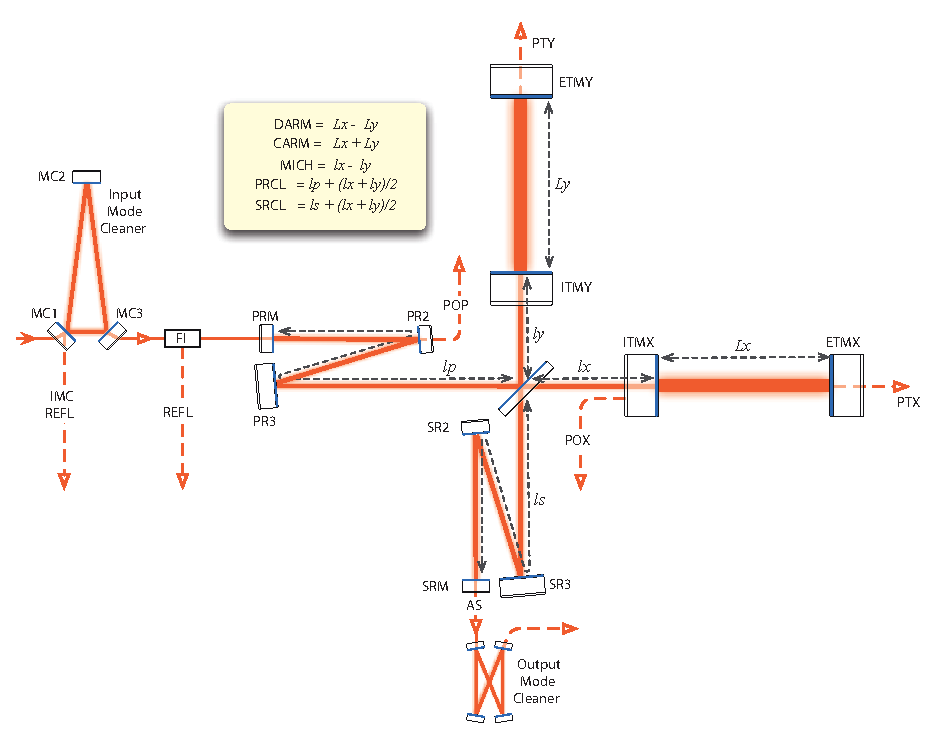
\includegraphics[width=0.8\textwidth]{Sec_Optics/aLIGO_IFO_Schematic}
\caption[Schematic optical layout of Advanced LIGO]
{Schematic drawing of the Advanced LIGO optical layout, degrees-of-freedom and sensing ports \cite{aLIGO_lscfdd}. 
Error signals for the control of the five longitudinal degrees-of-freedom are extracted from the four ports REFL, AS, POP and POX.}
\label{Fig:Sec_Optics_AdvLIGO_IFO_Schematic}   
\end{figure}

For Advanced LIGO different modes of operation are foreseen, each of them involving e.g.\ different input laser power levels, signal
recycling tunings, homodyne detection phases, etc., to yield optimum signal-to-noise ratio, depending on the astrophysical source under investigation~\cite{aLIGO_lscfdd}. 
The main differential control requirement for Advanced LIGO is $10^{-15}$\,m rms, yielding a shot noise limited sensitivity of $4 \times 10^{-21}$\,m/$\sqrt{\textnormal{Hz}}$.

At the detector's operating point the carrier laser light is resonant in the power recycling cavity (PRC) and in the arm cavities. The signal recycling cavity (SRC)
is tuned to carrier resonance only if the detector is operated in tuned mode. 
Two pairs of phase modulation sidebands, locked by a PLL, are imprinted on the input laser, forming the basis of the sensing scheme. 
The frequencies were chosen to be $f_1=9$\,MHz and $f_2=45$\,MHz, both nearly anti-resonating in the arms to reduce arm-cavity induced phase shifts.%\footnote{This turns out
%to have a positive effect on the shot noise sensitivity of the Michelson (MICH) degree-of-freedom.} 
Both pairs of modulation sidebands are resonant in the power recycling cavity. The signal recycling cavity, however, is arranged to be nearly resonant for the $f_2$ sidebands 
while the $f_1$ sidebands do not resonate.

A typical property of the recycling cavities is their potential to cause mixing of modulation sidebands which immediately leads to 
coupled error signals. To prevent this effect from rendering the control scheme more complicated than necessary it is crucial to 
arrange for a configuration that reduces this mixing to the largest possible extent. 

The Schnupp asymmetry---a macroscopic offset in the arm lengths of the central Michelson---is set to 5\,cm to provide nearly critical coupling of the $f_2$ 
sidebands in the dual recycling cavity, with the implication of simultaneous resonance of the power recycling and the signal recycling cavities 
for this sideband frequency. By choosing an appropriate value for the Schnupp asymmetry one can arrange for a large modulation sideband power ratio in the SRC, 
providing improved signal separation. In this case the resulting power ratio is of the order of $10^3$, in favor of the $f_2$ sidebands.

A variety of ports in the interferometer are read out to obtain a complete set of control signals for all longitudinal degrees-of-freedom. 
Besides the asymmetric port (AS), signals are extracted from the symmetric port (REFL) and from pick-off ports from within the power recycling cavity (POP)
and a in reflection of one of the arm cavities (POX). These beams are directed to photodetectors and the resulting signals are in 
turn demodulated at $f_1$, $f_2$, $f_2-f_1$ or $f_1+f_2$, at appropriately set demodulation phases. 
Demodulation at the sum or difference frequency of two modulation sidebands, i.e.\ at their beat frequency, is a key concept in modern interferometric control system design and is 
often referred to as \emph{double demodulation}.

The signal obtained in the symmetric port, after demodulation at the lower sideband frequency $f_1$ is used for common mode arm cavity (CARM) control. 
Consequently, the differential arm cavity mode control signal is obtained in the asymmetric port from the AS DC photodetector. For the DC readout scheme 
of the asymmetric port, which also contains the GW signal, a differential arm length (DARM) offset of the order of $10^{-11}$\,m will be applied, yielding a DC power level in 
the asymmetric port of the order of $0.1$\,W of carrier light.
The intra-cavity POP port yields signals for the PRC and the Michelson degrees-of-freedom, after demodulation at
$f_1$ and $f_2$, respectively. 

For controlling the signal recycling cavity, the optimum signal extraction port as well as the demodulation frequency depends on the mode of operation, i.e.\ the tuning 
of the SR cavity. Whereas for zero detuning an appropriate error signal can be extracted in the symmetric port in reflection of the
interferometer or at the arm cavity pick off port, for detuned operation analyses have shown that double demodulation of the asymmetric port signal
yields better error signals. Thus, if it is desired to continuously tune the SR from tuned mode to a detuned science mode, at a detuning of about
5 deg it is necessary to switch between error signals for the control of the signal recycling cavity.

The underlying sensing matrix shows well-separated error signals for the arm cavities' degrees-of-freedom. The power recycling cavity is sufficiently decoupled from the other degrees-of-freedom
but shows strong coupling to the ports where the Michelson and signal recycling cavity error signals are obtained. The most worrisome degrees-of-fredom are the differential arm length of the central Michelson interferometer (MICH) and the signal recycling
cavity length which exhibit comparably large amount of cross-coupling. However, control of the interferometer can be gained e.g.\ with a gain hierarchical approach in conjuction with the arm length stabilization system (ALS) which
is discussed in Sec.~\ref{sec:detector_lock_acquisition}.

The control signals derived from the error signals are applied to the end mirrors in the case of the DARM degree-of-freedom, to the beamsplitter for differential arm length of the central Michelson feedback  and to the recycling
mirrors for SRC and PRC length stabilization. However, the common mode arm cavity length control loop is the most elaborate one. The CARM error signal is fed back to the main laser via multiply cascaded
frequency loops, providing the final level of frequency correction.
The required unity gain frequencies of the servo controllers are of the order of tens of Hz for PRC, SRC and MICH, hundreds of Hz for 
DARM and tens of kHz for the CARM degree-of-freedom. 

With the exception of the arm cavity common mode controller all servo loops are realized using digital controls.
The more demanding (in terms of bandwidth) CARM servo will be implemented in analog electronics.
The digital feedback loops are implemented in a custom-made real-time control system with typical sampling rates of up to
65536 samples per second at up to 18 bit resolution. Digital control systems have proven to be a powerful solution with high flexibility. 
Complex filter structures, e.g.\ with blending of sensors and signals, can be conveniently realized and changed on-the-fly with little effort.

Similar to the initial LIGO control scheme, correction paths are included in the Advanced LIGO scheme. Correction signals are filtered 
copies of sensing noise limited MICH and SRCL control signals. To cancel the effects of known couplings, correction signals are fed
from SRCL to DARM and from MICH to DARM at a precision of 1\%. An additional correction path will feed signals from PRCL to DARM, at
a lower precision of 10\%.
\FloatBarrier
\paragraph{Detector lock acquisition}\label{sec:detector_lock_acquisition}
Lock acquisition is the process of bringing an interferometer from its uncontrolled, initial state to a controlled state in which the instrument
is fully operable. 
Contrasting the case of a servo loop operating near resonance, where the error signal for an optical cavity shows a linear response to length changes, during lock acquisition one has
to generally deal with highly nonlinear signals. Servo loops are usually optimized for control on resonance, resulting in a poor performance during acquisiton.
The determining quantity in lock acquisition of an optical cavity system are the mirrors' relative velocities. Further, the \emph{threshold velocity} 
is usually referred to as a measure which quantifies the performance of an acquisition scheme. By definition the threshold velocity is the maximal relative velocity of 
two cavity mirrors below which lock acquisition is successful. The threshold velocity strongly depends on the bandwidth of the underlying control loop.
Only if the servo response time is suffiently short to follow the transient error signal it is capable of ``capturing'' an optic.
As the probability for all DOF being simultaneously at their operating points is very small, a sequential approach must be taken, bringing the DOF to the locked state one after another.

The simplistic approach to lock acquisition, e.g.\ practiced in the early detector prototypes, is to wait for the instrument's DOF, driven by random ground motion, to move close to their operating points and then swiftly engage
the control loops. As with this method lock acquisition of an interferometric GW detector would be a pure matter of coincidence more deliberate approaches were strongly desired.
For initial LIGO an acquisition algorithm was developed which is based on a real-time estimate of the time-evolving sensing matrix, derived from measurable signals during lock acquisition \cite{EMFBBGKLSW02}.
With the implementation of this scheme on the LIGO digital control and data system lock of the detector was on average acquired on timescales of $\sim1$\,min. 
The Virgo approach to lock acquisition was to effectively decouple the instrument's DOF which is achieved by a deliberate misalignment of optics. This technique is often referred to as \emph{variable 
finesse locking} \cite{Virgo_VariableFinesse06}. Lock was usually acquired within a few minutes. 

The Advanced LIGO quadruple suspensions provide isolation to the test masses with respect to ground motion at frequencies above 10\,Hz.
Even though the active internal seismic isolation (ISI) platforms provide additional low frequency isolation, low frequency disturbances are
expected to cause significant test mass displacement of the order of $10^{-7}$m/$\sqrt{\textnormal{Hz}}$ at 0.5\,Hz. This is due to the fact that at 
the suspension system's resonance frequency or at lower frequency perturbations are not well attenuated and couple into the test masses' positions as displacement noise.
Besides this, the test masses will have electrostatic actuators instead of coil-magnet actuators which were used in initial LIGO. Electrostatic actuators deliver
lower actuation noise, at the expense of significantly lower actuation force they can exert on the test masses. The Advanced LIGO electostatic actuators are expected to
saturate at forces of $\sim200\,\mu$N \cite{LIGO_T1000294}. This severely complicates the process of lock acquisition.

In order to ease the difficulties of lock acquisition in the Advanced detector generation, auxiliary laser based schemes will be employed to complement the well-established techniques.
This discussion focusses on the Advanced LIGO ALS (arm length stabilization) system \cite{aLIGO_ALS_Design}. For Advanced Virgo it is anticipated to employ a similar scheme. 
Other systems to aid lock acquisition, that were considered for use in Advanced LIGO, such as the suspension point interferometer or digital interferometry are described in \cite{LIGO_T080139}.
The underlying idea of ALS is to provide for more deterministic lock acquisition by locking the arm cavities independently of the remaining degrees-of-freedom.
The ALS system builds on frequency doubled laser beams launched into the arm cavities through the end test masses for pre-stabilization of the interferometer arms,
independent of the science laser circulating in the interferometer. By applying additional coatings on the arm cavity mirrors the properties of the arm cavities, 
as seen from the ALS, can be shaped in accordance to the pre-stabilizations scheme's requirements. The choice of reflectivities for the input mirror and the end mirror 
results in an overcoupled cavity for the auxiliary laser, seen from the end mirror. The Finesse of the arm cavities for the 532\,nm ALS beams is $\sim100$. 
A simplified schematic of the ALS principle setup is depicted in Fig.~\ref{Fig:Sec_Optics_AdvLIGO_ALS_Schematic}.

\begin{figure}[th]
\centering
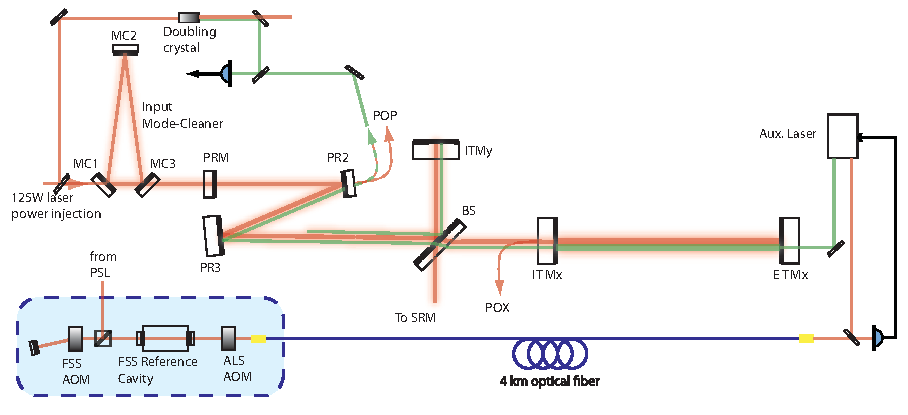
\includegraphics[width=0.8\textwidth]{Sec_Optics/aLIGO_ALS_Schematic}
\caption{Schematic drawing of the Advanced LIGO arm length stabilization (ALS) subsystem \cite{aLIGO_ALS_Design}. The test mass motion is reduced prior to lock acquisition by a combined scheme
of PDH reflection locking of an auxiliary laser to the arm cavities and hetorodyne detection of the transmitted beams. The optical fiber is necessary to provide an optical reference at the end 
stations, to lock the auxiliary lasers' phases to the science laser.}
\label{Fig:Sec_Optics_AdvLIGO_ALS_Schematic}   
\end{figure}

The initial step in the acquisition process is to hold the arm cavities on anti-resonance for the main science laser. In the next step the 
recycling cavities are brought to the locked state, before the ALS brings the arm cavities onto resonance with the main laser and
hands over the control authority to the global interferometer sensing and control scheme. For effectiveness, the ALS must reduce the residual
arm cavity length fluctuations to a displacement of no more than one cavity line width, which is approx. 1.3\,nm in the case of the
Advanced LIGO arm cavities. Estimations have shown that with ALS engaged a level of displacement fluctuations of 0.115\,nm rms can be 
reached. 

Technically, once the arm cavities are locked with the 532\,nm beams, a heterodyne measurement is performed on the ALS beam transmitted by 
the x-arm cavity and a frequency doubled sample of the main laser beam. A second one is performed between the x-arm and the y-arm transmitted beams. These measurements 
yield common and differential mode error signals which are in turn fed back to the corresponding actuators. By introducing a tunable offset
into the heterodyne locking loop, the arm cavities can thus be adjusted to arbitrary tunings.

For a smooth transition from ALS arm cavity control to global control a robust phase-locked loop (PLL) is crucial, to provide a well-defined phase relationship
between auxiliary lasers and the main science laser. Once the PLL is closed, the auxiliary lasers are locked to the arm cavities using PDH reflection locking. The resulting control signal
acts on a voltage-controlled oscillator (VCO) which supplies the electronic local oscillator for the PLL. In this way the offset frequency of the auxiliary laser with
respect to the reference is tuned. An analog servo is foreseen for this loop and is expected to have a bandwidth of a few kHz.

To provide a stable frequency standard for the auxiliary laser PLL, a technique based on the LISA (Laser Interferometer Space Antenna) back-link measurement is employed. Mullavey et al. \cite{MSSM10}
have experimentally demonstrated a scheme based on counter propagating two laser beams through an optical fiber and subsequent measurements of each of the 
outputs with LISA-style phasemeters. By subsequent combination of the output signals an error signal can be obtained which can be utilized to eliminate fiber induced phase noise. Their setup 
consisted of 4.6\,km single mode optical fiber and two Nd:YAG lasers---operated in a master-slave configuration. To circumvent
nonlinear forms of noise such as stimulated Brillouin scattering, the transmitted laser power was reduced to $\sim50\,\mu$W.
In the underlying bench top experiment a relative frequency noise of 0.5\,mHz/$\sqrt{\textnormal{Hz}}$ was reached for Fourier frequencies between 5\,Hz and 20\,Hz which is
well below the Advanced LIGO requirements, with a margin of more than an order of magnitude.


%\section{Introduction}

%The detection principle of a large scale gravitational wave interferometer is to sense the passage of a gravitational wave as a light intensity change at the asymmetric interference port  due to the phase shift in the long arms. 
%This is possible only if the test masses are suspended well enough to be considered as \emph{free-falling test masses}.\\
% Such instruments provide  useful signal only when the optical components are positioned precisely at  pre-defined locations relative to each other (to have the long cavities resonating and a destructive interference at the beam splitter).
% This set of positions is called the \textit{operating point}.\\
% Sophisticated electro-optical feed-back control systems are required to continuously measure and restore the
% mirror positions. Two separate systems to control the mirror position are used: one for the
% longitudinal position along the optical axis, and the other for the angular positions 
% of the mirrors.
\FloatBarrier
\paragraph{Angular control - Automatic Alignment control system}%\label{sec:asc}

The angular control system has to be implemented in order to reduce the mirror misalignments 
in the frequency region in which the seismic attenuation system does not fulfill the alignment
requirements, i.e.\ below the mechanical resonances, to reduce  the fluctuations of the mirror 
angular positions with respect to the beam,  to maintain the overall alignment of the optical elements, 
ensuring long data taking periods, and to reduce the noise at the output
port.
The mirror angular positions in data taking mode can not be locally controlled because the long term 
drifts of the local references spoil the overall alignment.  
After the lock has been acquired the angular control has to be switched to a global control system, the
 \textit{Automatic Alignment},  which uses error signals derived from the interferometer itself with a
 modulation-demodulation technique based on differential wave front sensing.
The control scheme chosen for the second and third generation of gravitational wave interferometer
 is a Ward-like scheme where the RF modulation frequencies are chosen to do not have any 
  higher order modes resonating in the cavities~\cite{ward}.

The main differences between the third generation and the first generation of gravitational wave
 detectors,  relevant for alignment control are: 
 \begin{itemize}
 \item presence stable recycling cavities
 \item higher circulating power
 \item presence of  signal recycling
 \end{itemize}
These modifications will provide an improvement of the overall interferometer stability and sensitivity but also 
increase of complexity for the  Automatic Alignment control system.

\textbf{Stable Recycling cavities issue}

The stable recycling cavities aim to make the potential higher order modes content to be less affected by 
 thermal effects in the mirrors. This behaviour influences the Automatic Alignment control system since the amplitude of 
the alignment error signals is proportional to the amount of the TEM$_{01/10}$ modes. 
For example in the case the recycling cavity with a Gouy phase of 15~deg the TEM$_{01}$ mode is attenuated
 by a factor of about 6 while for 25~deg the attenuation factor is about 9.
For this reason the choice of the recycling cavity Gouy phases has to be done taking into account both the 
stability requirements and the amount of first order higher order modes to ensure the angular controllability of the system. 
 
 
\textbf{High circulating power issue} 

In an high power interferometer \textit{radiation pressure} plays an important role. The light beam acts on the mirror 
such as an optical spring whose strength increases with the power. This effect will be largest in the Fabry-Perot arm cavities,
but the effect has also to be  evaluated for the mirrors of  the central
 interferometer.  

Due to radiation pressure the two cavity mirrors
 become coupled and their angular motion must be described in terms of two linear combinations \cite{sidles-sigg}. 
When the circulating power becomes large enough one of the angular modes can become dynamically unstable. 
As derived in \cite{sidles-sigg}, the interaction of the beam and the mirrors can be written in term of the stiffness matrix:
\begin{equation}
\mathbf{k} = \frac{2PL}{c(1 - g_1 g_2)} \left[ \begin{array}{cc} -g_2 & 1 \\ 1 & -g_1\end{array}\right]
\end{equation}
where $g_i = 1 - L/R_i$ are the G-factors of the two mirrors. The eigenvectors and eigenvalues of the stiffness matrix 
determine the physical angular degrees of freedom and the corresponding stiffness applied to the mechanical system. 

The normal stable situation corresponds to a positive stiffness of the system, given by the contribution of the mechanical 
stiffness of the mirror suspension and the extra-stiffness due to the radiation pressure, which gives a resonance made of
 a pair of complex poles with negative real part and quite large quality factor. The case of negative stiffness instead leads
 to an unstable system described with two real poles, one with positive and one with negative real part, with very close absolute frequency.
The radiation pressure effects have then to be taken into account in the design of the control system.


Moreover the presence of the Signal Recycling mirror increases the number of degrees of freedom to control with respect
 the first generation of gravitational wave interferometers.

The design of the Automatic Alignment control system will be challenging because of the above mentioned issues and of 
the control accuracy and noise requirements to reach the targeted ET sensitivity.
On the other hand all these effects and potential issues will be studied for the commissioning of the second generation 
interferometers, such as Advanced Virgo and Advanced LIGO, and therefore providing plentiful  experience 
how to mitigate these difficulties.



\subsubsection{Thermal effects and their compensation}\label{sec:tcs}
%\emph{Author(s): V.\ Fafone, A.\ Rocchi \\}

Thermal lensing due to the absorption of the laser light in the core optics of gravitational wave interferometers can represent a  limitation for 
 their operational stability and sensitivity. This effect has already been observed in the currently operating
  detectors (requiring the installation of compensation systems~\cite{ligotcs,virgotcs,Accadia2010}) and 
  will become more relevant in the second generation interferometers, due to the much higher circulating power. 
In case of ET xylophone configuration with a low-frequency cryogenic and
 a high-frequency room-temperature detector, the two interferometers show a different behaviour with respect to thermal effects. 

Due to the low power circulating in the Fabry-Perot cavities  and due to the thermal properties of silicon 
at low temperature (see table~\ref{tab:tn_T_param}), thermal effects in ET-LF will be negligible: the thermal 
gradient due to the laser power absorption results to be less than 1\,mK. On the contrary, the ET-HF 
interferometers will feature all the characteristics of an advanced detector (room temperature operation, 
high power and fused silica test masses, similar arm cavity finesse and recycling gains) and the only difference is
 the application of a LG$_{33}$ beam profile instead of TEM$_{00}$. 

In the test masses, the optical power is predominantly absorbed by the high-reflectivity 
coatings and converted into heat, producing a temperature gradient 
inside the substrate. While R\&D activities to reduce coating absorptions are ongoing (see Sec.~\ref{sec:RD}), 
values of about 0.6\,ppm have been reported in literature~\cite{pin09}. Thus, considering 3\,MW of optical 
power impinging on the test masses, the total absorbed power amounts to 1.8\,W. This is a factor of three higher than expected 
in advanced detectors~\cite{fafo08}. However, the resulting maximal temperature increase is less than 
1~degree, as shown in figure~\ref{Fig:Sec_Optics_TCS1}, compared to about 2 degrees in the advanced detectors.
 This result is mainly due to the wider intensity distribution of the LG$_{33}$.
 % in fact, in advanced detectors, where the power inside the Fabry-Perot cavities will be around 800\,kW, lower
 % by more than a factor of three than in ET-D-HF, but a TEM$_{00}$ will be used, the temperature increase is 
 %expected to be of the order of 2 degrees with the same coating absorption level~\cite{fafo08}. 
 By integration of the temperature field along the thickness of the test mass, it is possible to calculate the
  corresponding optical path length (OPL) increase. In figure~\ref{Fig:Sec_Optics_TCS2} the expected ET-HF
   optical path increase is compared to the expectation for Advanced Virgo~\cite{fafo08}: the use of LG$_{33}$ 
   modes will limit the increase of thermal effects with respect to advanced detectors to about 30\%.

\begin{figure}[!h]
\centering
\includegraphics[width=0.4\textwidth]{Sec_Optics/TCS_1b}
\caption{Temperature distribution in ET-D-HF test mass due to the absorption of 0.6\,ppm of the arm cavity power.}
\label{Fig:Sec_Optics_TCS1}   
\end{figure}

%\textcolor{red}{Comment for the TWT: coating absorption only accounted for: FP cavity finesse and RC cavity gain needed to evaluate substrate contribution. If these parameters are not yet defined, we will add a sentence specifying the approximation used in the evaluation of thermal effects.}

\begin{figure}[!h]
\centering
\includegraphics[width=0.45\textwidth]{Sec_Optics/TCS_2}
\caption{Optical path length (OPL) increase in ET-HF test mass (blue curve) compared to the expected values for Advanced Virgo (green curve).}
\label{Fig:Sec_Optics_TCS2}   
\end{figure}

%\subsubsection{CO$_2$ laser correction}
%\label{sec:tcs1}
%\vspace{1cm}

Since the thermal effects expected for ET-HF are  of the same order of magnitude as the ones expected for advanced detectors,
it will possible to apply for ET the same thermal compensation system (TCS) as adopted for 2$^{nd}$ generation
  interferometers. ET-HF could use a compensation plates (CP) in the recycling cavity, heated by CO$_2$ lasers,
   to cope with thermal lensing and a ring heater around each test mass to correct its thermally driven increase of radius of 
   curvature. Figure~\ref{Fig:Sec_Optics_TCS3} shows a sketch of a compensation plate  and a ring heater  around the test mass. 

\begin{figure}[!h]
\centering
\includegraphics[width=0.35\textwidth]{Sec_Optics/TCS_3.png}
\caption{Sketch of the ET compensation plate and ring heater around the test mass (not in scale).}
\label{Fig:Sec_Optics_TCS3}   
\end{figure}

%In figure~\ref{Fig:Sec_Optics_TCS3}, the CP is thinner than the test mass. This is done to minimize the loss of compensating power from the barrel of the CP~\cite{fafo10}. On the other hand, the thickness cannot be reduced at will, since it is necessary to accumulate enough optical path lenght increase. For instance, in Advanced Virgo the CP will be 3.5\,cm thick. A reduction of the heat loss could also be achieved by gold coating the barrel of the CP (provided that the mechanical quality factor of the CP is not reduced too much).

%Since the radiative coupling between the input test mass and the compensation plate spoils the efficiency of the TCS~\cite{fafo10}, from the point of view of the thermal effects compensation, the best scheme is to suspend the CP "far" from the test mass, at a distance that minimizes the radiative coupling. 
%This would also allow to mechanically de-couple the CP from the ITM payload. 

In order to optimize the compensation level, the CP heating pattern must  account for the intensity profile of the interferometer beam. 
%will use LG$_{33}$ modes. 
A heating pattern optimization code has been developed~\cite{rocchi10}, consisting of a linear iterative optimization process based on a finite element 
analysis,
that makes use of the OPL increase ($\Delta \text{OPL}$) as error signal. At each iteration, the heating 
 pattern for the next step is calculated from the previous one and from the corresponding OPL increase:
\begin{equation}
H_{\text{path}}(n+1)=H_{\text{path}}(n)+K_L \cdot  \Delta \text{OPL}(n),
\end{equation}
where, $H_{\text{path}}$ is the CP heating pattern and $K_L$ is the loop gain. The procedure is applied 
to the complete system made of the test mass, the compensation plate and ring heater.
The result, when the compensation plate is placed sufficiently ``far'' from the ITM (thus there is no significant
radiative coupling between the test mass and the compensation plate), is shown in Fig.~\ref{Fig:Sec_Optics_TCS4}. With this 
heating pattern, TCS can flatten the optical path lenght inside the input test mass substrate up to a diameter 
of 40\,cm. This heating profile could be produced, for example, using scanning systems ( for instance making  use of  galvos
 or crossed AOMs).%, diffractive optical elements or MEMS.

\begin{figure}[!h]
\centering
\includegraphics[width=0.7\textwidth]{Sec_Optics/TCS_4c.png}
\caption{Left picture: optimized heating pattern. Right picture: compensated optical path length (green curve) compared to the uncompensated one (blue curve).}
\label{Fig:Sec_Optics_TCS4}   
\end{figure}

Since the ET infrastructure will comprise cryogenic facilities, it could be possible to exploit them to implement a
 different technique for the compensation of thermal effects.
Such a system would aim to directly extract the heat deposited by the laser beam, before it has a chance to generate any deformation of
 the mirror. Localized heat extraction can be implemented via directional radiative cooling of the beam spot~\cite{kamp2009}. 
 For this it is required  to image a sufficiently cold black
body on the beam spot (but not on
the rest of the mirror), from a sufficiently large solid angle. Figure~\ref{Fig:Sec_Optics_TCS6} shows a conceptual design of the system.

\begin{figure}[!h]
\centering
\includegraphics[width=0.3\textwidth]{Sec_Optics/TCS_6.pdf}
\caption{Conceptual scheme of the radiative cooling.}
\label{Fig:Sec_Optics_TCS6}   
\end{figure}

%The heat extraction efficiency of the technique
%drops as $T^4$, thus becoming rapidly ineffective for mirrors cooled to
%cryogenic temperatures. For this reason, this method could be used only on the high frequency component of ET, since it is a room-temperature detector.

By placing parabolic collectors behind each cold spot, the radiative coupling with the mirror 
surface is improved and it is possible to achieve  a strong reduction of the required size of the cold spot~\cite{tvpi10}. 
Such a scheme, named \emph{parobolic mirrors radiative cooling}  is shown in figure~\ref{Fig:Sec_Optics_TCS7}. 
The role of each reflector-collector couple is to build up a telescope that enlarges the radiative exchange surface 
of the cold target,
as seen by the test mass center spot. This allows for the implementation of
small cold surfaces with low cooling power and efficient temperature control.
\begin{figure}[!h]
\centering
\includegraphics[width=0.4\textwidth]{Sec_Optics/TCS_7b}
\caption{Scheme of the Parabolic Mirrors Radiative Cooling.}
\label{Fig:Sec_Optics_TCS7}   
\end{figure}


The parobolic mirrors radiative cooling technique is being investigated~\cite{tvpi10} with the main aim of assessing the 
capability of the system in producing proper cooling profiles. This is done in a test facility that allows the
 imaging system and the shape of the cold spots to vary in order to modify the cooling profile and to take  the use of LG$_{33}$ modes in ET-HF
 into account.

The same concept of radiative cooling can be clearly applied to image a warm source (or an array of sources) to
 produce heating profiles onto the periphery of the test mass. This could allow us, in principle, to avoid using compensation 
 plates, provided that the noise injected by the heating system is compliant with the sensitivity requirements.

All these radiative techniques are at present under investigation. The CO$_2$ laser based 
TCS has already proven able to generate proper heating profiles.
% the radiative methods must be further studied to demonstrate their capability in producing compensating
% patterns with the accuracy required in next generations detectors. 
Again ET will be able to benefit from the vast experiences that will be gained 
by the commissioning of the TCS systems for Advanced Virgo and Advanced LIGO.

